\documentclass[pdftex,12pt,a4paper]{article}

\usepackage{wrapfig, amssymb, amsmath, graphicx, subfigure, pifont, seqsplit, float, booktabs, siunitx, adjustbox}
\usepackage[english]{babel}
\usepackage[top=1in, bottom=1in, left=1in, right=1in]{geometry}
\pagenumbering{arabic}
\newcommand{\HRule}{\rule{\linewidth}{0.5mm}}

\usepackage{forest}
\tikzset{el style/.style={midway, font=\scriptsize, inner sep=+1pt, auto=right}}
\forestset{angled/.style={
    content/.expanded={\noexpand\textless\forestov{content}\noexpand\textgreater}}}

\begin{document}
\begin{titlepage}

% Upper part of the page
\begin{flushleft}

\includegraphics[trim=0mm 0mm 0mm 0mm, width=1\textwidth]{./logo.jpg}\\
\end{flushleft}
\begin{center}
	\textsc{\Large Informatie en Communicatie}\\[0.5cm]

    % Title
    \HRule \\[0.4cm] { \huge \bfseries HW-1}\\[0.4cm]

    \HRule \\[1.5cm]

    % Author and supervisor
\begin{minipage}{0.4\textwidth}
\begin{flushleft} \large \emph{Authors:}\\
Abe \textsc{Wiersma}\\
\end{flushleft}
\end{minipage}
\begin{minipage}{0.4\textwidth} \begin{flushright} \large \end{flushright}\end{minipage}

    \vfill

    % Bottom of the page 
    {\large \today}

\end{center}
\end{titlepage}
\pagebreak

\begin{enumerate}
    \item
        \begin{enumerate}
            \item $H(f(Y)) ? H(Y)$\\
                \begin{align}
                    H(Y) &= H(Y) + H[f(Y)|Y]\\
                         &= H(Y,f(Y))\\
                         &= H(f(Y)) + H(Y|f(Y))\\
                         &\ge H(f(Y))\\
                 H(f(Y)) &\le H(Y)
                \end{align}
            \item $H(X|f(Y)) ? H(X|Y)$
                The entropy of $f(Y)$ only decreases or is equal to the
                entropy of $Y$
                \begin{figure}[h]
                \centering
                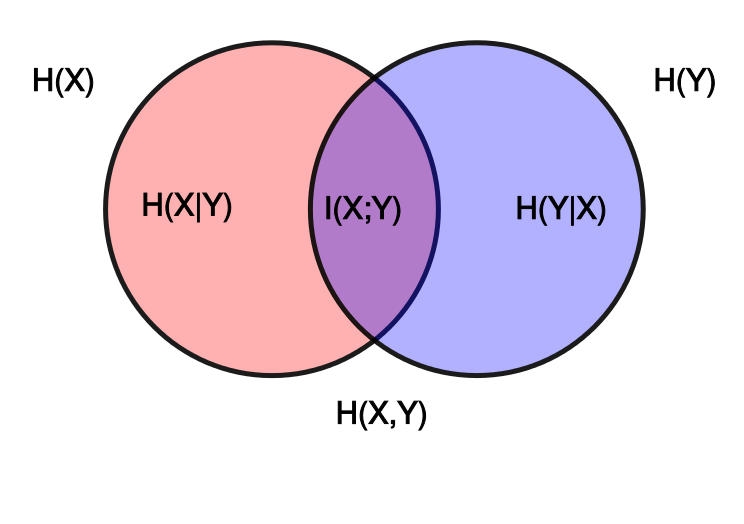
\includegraphics[width=0.5\linewidth]{venn.png}
                \end{figure}

                If H(f(Y)) is smaller than H(Y) this means:\\
                $H(X|Y) \ge H(X|f(Y))$\\
                $H(X|f(Y)) \le H(X|Y)$
            \item $I(X,Z|Y) = 0 \implies I(X;Z) ? I(X;Y)\mathrm{ \& }I(X;Z) ? I(Y;Z)$
                \begin{align}
                    I(X;Z|Y) &= I(X;Y,Z) - I(X;Y) = 0\\
                             &= I(X;Y|Z) + I(X;Z) - I(X;Y) = 0\\
                             &= I(X;Y|Z) + I(X;Z) = I(X;Y) \implies I(X;Z) \le I(X;Y)
                \end{align}
                \begin{align}
                    I(X;Z|Y) &= I(X;Y,Z) - I(X;Y) = 0\\
                             &= I(X;Y|Z) + I(X;Z) - I(X;Y) = 0\\
                             &= I(X;Z) = I(X;Y) - I(X;Y|Z)\\
                             \intertext{Chain rule for mutual information}
                             &= I(X;Z) = I(X;Y) - (I(X;Y) + H(Z|X) + H(Z|Y) - H(Z|X,Y) - H(Z))\\
                             &= I(X;Z) = - H(Z|X) - H(Z|Y) + H(Z|X,Y) + H(Z)\\
                             \intertext{$I(X;Y)= H(X,Y) - H(X|Y) - H(Y|X)$}
                             &= I(X;Z) + H(Z,Y) - H(Y|Z) = I(Z;Y) - H(Z|X) + H(Z|X,Y) + H(Z)\\
                             &= I(X;Z) + H(Z,Y) - H(Y|Z) + H(Z|X) - H(Z|X,Y) + H(Z) = I(Z;Y)\\
                             &= I(X;Z) + H(Z,Y) - (H(Y|Z) - H(Z)) + H(Z|X) - H(Z|X,Y) = I(Z;Y)\\
                             &= I(X;Z) + H(Z,Y) - H(Z,Y) + H(Z|X) - H(Z|X,Y) = I(Z;Y)\\
                             &= I(X;Z) + H(Z|X) - H(Z|X,Y) = I(Z;Y)\\
                             &= I(X;Z) - (-H(Z|X) + H(Z|X,Y)) = I(Z;Y)\\
                             &= I(X;Z) - (H(Z|X,Y) - H(Z|X)) = I(Z;Y)\\
                             &= I(X;Z) - H(Y|Z|X) = I(Z;Y)\\
                             &= I(X;Z) = I(Z;Y) + H(Y|Z|X)\\
                             &= I(X;Z) = I(Z;Y) + H(Y|Z|X) \implies I(X;Z) \ge I(Z;Y)
                \end{align}
                Too long but correct.
        \end{enumerate}
    \item For each statement below, specify a (different) joint distribution
        $P_{XYZ}$ of random variables $X$, $Y$ and $Z$ such that the
        inequalities hold.
        \begin{enumerate}
            \item There exists a $y$, such that $H(X|Y = y) > H(X)$\\
                Let (X,Y) take values on $(0,0), (0,1) (1,0)$ with equal
                probability $(p=1/3)$.\\
                Then $H(X)=h(1/3)\approx0.92 < 1$.\\
                But $H(X|Y=0)=h(1/2)=1$\\
            \item $I(X;Y) > I(X;Y|Z)$
                Let Z make X and Y independant.
                Let (X,Y) take values on $(0,0), (0,1) (1,0)$ with equal
                probability $(p=1/3)$.\\
                But (X,Y|Z) take on values $ (0,1) (1,0)$ with equal
                probability $(p=1/2)$.\\
                Then $I(X;Y|Z) = 0$ and $I(X;Y) \approx 0.6$
            \item $I(X;Y) < I(X;Y|Z)$
                Let Z make X and Y dependant.
                Let (X,Y) take values on $(0,1) (1,0)$ with equal
                probability $(p=1/2)$.\\
                But (X,Y|Z) take on values $ (0,1) (1,0) (1,0)$ with equal
                probability $(p=1/3)$.\\
                Then $I(X;Y|Z) \approx 0.6$ and $I(X;Y) = 0$
        \end{enumerate}
    \item \textbf{Bottleneck:} Suppose a Markov chain starts in one of n
        states, necks down to $k < n$ states, and then fans back to $m > k$
        states. Thus $X_1\to X_2\to X_3$.
        \begin{enumerate}
            \item Show that the (unconditional) dependence of $X_1$ and $X_3$
                is limited by the bottleneck by proving that $I(X_1;X_3) \leq \log k$.
            \item  Evaluate $I(X_1;X_3)$ for $k = 1$, and explain why no
                dependence can survive such a bottleneck. 
        \end{enumerate}
    \clearpage
    \item Which of the three relations $\le, \ge, =$ holds between the quantities
        H(A) and H(C)? Prove your answer.
        \begin{align}
            I(A;C|B) &= I(A;B|C)\\
            I(A;C,B) - I(A;B) &= I(A;C,B) - I(A;C)\\
            I(A;B) &= I(A;C)\\
            I(A;B) &= I(A;C) = 0\\
        \end{align}
        Both B and C are independent of A, so H(A) != H(C)
        H(Y|X)=0  if and only if the value of Y is completely determined by the
        value of X
        \begin{align}
            H(A|B,C) &= 0\\
        \end{align}
        A can only be fully decided by B,C if $B\le A$
\end{enumerate}

\end{document}
